% Artigo final do projeto de Engenharia de Confiabilidade (UFMG).
% IEEEtran conference (v1.8b), compilar com pdfLaTeX (Overleaf: Menu -> Compiler -> pdfLaTeX).
\documentclass[conference]{IEEEtran}

\usepackage[T1]{fontenc}
\usepackage[utf8]{inputenc}
\usepackage[brazil]{babel}
\usepackage{cite}
\usepackage{amsmath,amssymb,amsfonts}
\usepackage{graphicx}
\usepackage{textcomp}
\usepackage{xcolor}
\usepackage{booktabs}
\usepackage{url}
\usepackage{siunitx}
\sisetup{output-decimal-marker={,}, group-separator={\,}, group-minimum-digits=4, exponent-product=\times}
\usepackage{tikz}
\usetikzlibrary{positioning,calc}

% Dado que ainda depende da equipe (aparece em azul no PDF).
\renewcommand{\IEEEkeywordsname}{Palavras-chave}
\raggedbottom  % evita espaços esticados entre flutuantes e texto

\newcommand{\pendente}[1]{\textcolor{blue}{[#1]}}
% Taxas em falhas por 10^5 h.
\newcommand{\pcmh}{por $10^5$~h}

\begin{document}

\title{Análise Comparativa da Confiabilidade de Motores Aeronáuticos a Pistão, Turboélice e Turbofan}

\author{
\IEEEauthorblockN{Ana Amantea Leal Marques Afonso}
\IEEEauthorblockA{\textit{Engenharia de Sistemas} \\
\textit{Universidade Federal de Minas Gerais}\\
Belo Horizonte, Brasil \\
\pendente{ESCREVER: e-mail}}
\and
\IEEEauthorblockN{Bruno Lima Soares}
\IEEEauthorblockA{\textit{Engenharia de Sistemas} \\
\textit{Universidade Federal de Minas Gerais}\\
Belo Horizonte, Brasil \\
brunolima280103@gmail.com}
\and
\IEEEauthorblockN{Eduarda Amaral de Oliveira}
\IEEEauthorblockA{\textit{Engenharia de Sistemas} \\
\textit{Universidade Federal de Minas Gerais}\\
Belo Horizonte, Brasil \\
\pendente{ESCREVER: e-mail}}
\and
\IEEEauthorblockN{Mariana Pinho Barroso Sousa}
\IEEEauthorblockA{\textit{Engenharia de Sistemas} \\
\textit{Universidade Federal de Minas Gerais}\\
Belo Horizonte, Brasil \\
\pendente{ESCREVER: e-mail}}
\and
\IEEEauthorblockN{Victor Almeida Morais}
\IEEEauthorblockA{\textit{Engenharia de Sistemas} \\
\textit{Universidade Federal de Minas Gerais}\\
Belo Horizonte, Brasil \\
\pendente{ESCREVER: e-mail}}
}

\maketitle

\begin{abstract}
Em um avião monomotor, a falha do motor em voo elimina toda a propulsão.
Comparamos a confiabilidade de três tecnologias, representadas pelo Lycoming O-540 (pistão), pelo PT6A-34 (turboélice) e pelo CFM56-7B (turbofan), com diagramas de blocos de confiabilidade que incluem pares redundantes e falhas de causa comum.
A taxa total de cada motor vem da literatura, e a parcela de cada subsistema foi estimada em 1109 achados de componente de 2899 falhas de motor investigadas pelo NTSB entre 2008 e 2026.
Em um voo de 1~h, o motor a pistão falha com probabilidade de $1{,}24\times10^{-4}$, 83 vezes a do turboélice e 62 vezes a do turbofan.
A separação resiste a toda a faixa publicada.
No pistão, cilindros, válvulas, pistões e virabrequim respondem por 60\% das falhas, enquanto os magnetos duplicados ficam com 0,6\%; nas turbinas, compressores e turbinas lideram.
Os pares redundantes reduzem em cerca de 10 vezes a chance de perder a função, ganho limitado pela fração de causa comum $\beta$.
Dois motores a pistão só superam um turboélice se menos de 1,2\% das falhas forem comuns aos dois motores; contra o turbofan, o limite é 1,6\%.
No NTSB, 43\% das falhas de motor registradas em multimotores a pistão tiveram vítima fatal, contra 11\% nos monomotores a pistão e 3\% nos turboélices monomotores.
Um teste caso-controle com o tempo desde a revisão de 903 motores a pistão dá forma de Weibull 0,99, compatível com a taxa constante.
\end{abstract}

\begin{IEEEkeywords}
confiabilidade, motores aeronáuticos, diagrama de blocos de confiabilidade, falha de causa comum, desligamento em voo
\end{IEEEkeywords}

\section{Introdução}\label{sec:intro}

Em um avião monomotor, não há redundância para a propulsão.
Se o motor falha em voo, a aeronave passa a planar e o piloto precisa encontrar onde pousar.
O risco depende da tecnologia do motor.
Em aviões leves na Austrália, o Australian Transport Safety Bureau (ATSB) registrou entre 12 e 13 falhas ou maus funcionamentos \pcmh{} de motores a pistão~\cite{atsb2016}, enquanto os números publicados para turbinas ficam abaixo de 1 \pcmh{}~\cite{stobie2019,cfr25k,easa2017}.
Parte da explicação está na arquitetura: o motor a pistão depende de muitas peças em movimento alternado e de subsistemas em série, e a turbina trabalha em rotação contínua, com mais redundância no controle.

Esses números, porém, são publicados como uma taxa única para o motor inteiro.
Eles não mostram quais subsistemas concentram as falhas, nem permitem avaliar se a redundância, dentro do motor ou na instalação de dois motores, compensa uma tecnologia menos confiável.
Para responder a essas perguntas, é preciso modelar o motor como um sistema.

Este trabalho compara a confiabilidade de motores a pistão, turboélice e turbofan por meio de diagramas de blocos de confiabilidade (RBD, \emph{reliability block diagram}).
Os objetivos específicos, definidos na proposta do projeto, são:
(i)~representar a arquitetura de cada motor em um RBD;
(ii)~estimar a taxa de falha $\lambda$, o tempo médio entre falhas (MTBF) e a confiabilidade $R(t)$ de cada um;
(iii)~avaliar o efeito das redundâncias, isto é, da ignição duplicada no pistão, do controle eletrônico de dois canais no turbofan e do uso de dois motores na mesma aeronave;
e (iv)~identificar os subsistemas que mais contribuem para a falha de cada tecnologia.

Além de responder a esses objetivos, o trabalho mede as frações de cada subsistema em três bases públicas, calcula o valor da causa comum entre motores a partir do qual dois motores a pistão deixam de ser mais seguros que um a turbina e confronta o modelo com a proporção de falhas de motor que terminaram em acidente no Brasil.

\section{Revisão da Literatura}\label{sec:revisao}

As ferramentas clássicas de confiabilidade já foram aplicadas a sistemas de propulsão, mas quase sempre com pouca informação de campo.
Christenson \emph{et al.}~\cite{christenson2000} descrevem o uso de FMEA, árvore de falhas (FTA) e RBD no projeto de sistemas de propulsão aeroespacial e apontam a falta de dados como a principal limitação.
O trabalho mais próximo do nosso é o de Samuel \emph{et al.}~\cite{samuel2006}, que montaram um RBD em série de um turboeixo a partir de registros de campo, depois de identificar os modos de falha e limpar os dados.
Laskowski~\cite{laskowski2015} usou FTA em um motor marítimo; nenhum desses estudos compara tecnologias de motor no mesmo modelo.

Para as redundâncias, o modelo do fator $\beta$ separa da taxa de cada unidade a parcela de causas comuns, que derrubam as duas unidades ao mesmo tempo~\cite{ebeling1997,rausand2004}.
Com um só parâmetro, ele se presta a casos sem dados para estimar a dependência, como este.
Bobbio \emph{et al.}~\cite{bobbio2001} mostraram que uma árvore de falhas pode ser convertida em rede bayesiana sem perda de informação, o que abre a inferência diagnóstica (dada a falha, qual a causa) e a atualização de parâmetros com dados.

Os dados de falha disponíveis têm naturezas diferentes para cada tecnologia.
Para motores a pistão, o ATSB analisa os modos de falha~\cite{romeyn2007} e publica taxas por fabricante para aviões leves entre 2009 e 2014~\cite{atsb2016}.
Para turbinas, os números mais citados são limites regulatórios, como o de desligamentos em voo (IFSD) para operações ETOPS~\cite{cfr25k} e o de perda de potência para monomotores a turbina em voo por instrumentos (SET-IMC)~\cite{easa2017}.
Um limite diz quanto o motor pode falhar, e não quanto ele falha; tomá-lo como taxa subestima a vantagem da turbina.
Taxas observadas existem para o PT6~\cite{stobie2019} e para o CFM56-7B~\cite{cfm2012}, esta última divulgada pelo próprio fabricante.

Nenhuma dessas fontes distribui a taxa entre subsistemas.
Para isso, usamos bases de ocorrências: o Service Difficulty Reporting System (SDRS) da FAA~\cite{sdrs}, os achados de acidentes do NTSB~\cite{ntsb} e os relatórios do Centro de Investigação e Prevenção de Acidentes Aeronáuticos (CENIPA)~\cite{cenipa}.
Sem horas voadas, elas permitem estimar proporções, mas não taxas absolutas.

\section{Materiais e Métodos}\label{sec:metodos}

\begin{figure*}[t]
  \centering
  \resizebox{\textwidth}{!}{% Diagramas de blocos de confiabilidade (RBD) dos três motores. Blocos empilhados: par redundante.
\begin{tikzpicture}[
  font=\scriptsize,
  blk/.style={draw, rounded corners=1pt, align=center, minimum height=6.6mm, inner sep=1.5pt, text width=#1},
  blk/.default=12mm,
  rot/.style={font=\footnotesize\bfseries, anchor=east},
  >=stealth, line width=0.4pt]
\def\g{2.2mm}
% ---------------- Pistão ----------------
\node[rot] (lp) at (0,0) {Pistão};
\node[blk=11mm, right=\g of lp] (p1) {Admissão};
\coordinate[right=\g of p1] (p2i);
\node[blk=11mm, right=\g of p2i, yshift=4.6mm] (p2a) {Bomba mecânica};
\node[blk=11mm, right=\g of p2i, yshift=-4.6mm] (p2b) {Bomba elétrica};
\coordinate (p2o) at ($(p2a.east |- p2i)+(\g,0)$);
\node[blk=13mm, right=\g of p2o] (p3) {Carburador / injeção};
\coordinate[right=\g of p3] (p4i);
\node[blk=11mm, right=\g of p4i, yshift=4.6mm] (p4a) {Magneto 1};
\node[blk=11mm, right=\g of p4i, yshift=-4.6mm] (p4b) {Magneto 2};
\coordinate (p4o) at ($(p4a.east |- p4i)+(\g,0)$);
\node[blk=19mm, right=\g of p4o] (p5) {Cilindros, válvulas, pistões, virabrequim};
\node[blk=13mm, right=\g of p5] (p6) {Lubrificação};
\node[blk=15.5mm, right=\g of p6] (p7) {Arrefecimento};
\node[blk=13.5mm, right=\g of p7] (p8) {Hélice e governador};
\draw (p1) -- (p2i) |- (p2a); \draw (p2i) |- (p2b);
\draw (p2a) -| (p2o); \draw (p2b) -| (p2o); \draw (p2o) -- (p3);
\draw (p3) -- (p4i) |- (p4a); \draw (p4i) |- (p4b);
\draw (p4a) -| (p4o); \draw (p4b) -| (p4o); \draw (p4o) -- (p5);
\draw (p5) -- (p6) -- (p7) -- (p8);
% ---------------- Turboélice ----------------
\node[rot] (lt) at (0,-1.75) {Turboélice};
\node[blk=10mm, right=\g of lt] (t1) {Entrada de ar};
\node[blk=13mm, right=\g of t1] (t2) {Compressor};
\node[blk=13mm, right=\g of t2] (t3) {Câmara de combustão};
\node[blk=17mm, right=\g of t3] (t4) {Turbinas (compressor e livre)};
\node[blk=11mm, right=\g of t4] (t5) {Caixa de redução};
\node[blk=13.5mm, right=\g of t5] (t6) {Hélice e governador};
\node[blk=13mm, right=\g of t6] (t7) {Combustível (FCU)};
\node[blk=13mm, right=\g of t7] (t8) {Lubrificação};
\draw (t1) -- (t2) -- (t3) -- (t4) -- (t5) -- (t6) -- (t7) -- (t8);
% ---------------- Turbofan ----------------
\node[rot] (lf) at (0,-3.35) {Turbofan};
\node[blk=7mm, right=\g of lf] (f1) {Fan};
\node[blk=15.5mm, right=\g of f1] (f2) {Compressores LP e HP};
\node[blk=13mm, right=\g of f2] (f3) {Câmara de combustão};
\node[blk=12mm, right=\g of f3] (f4) {Turbinas HP e LP};
\coordinate[right=\g of f4] (f5i);
\node[blk=11mm, right=\g of f5i, yshift=4.6mm] (f5a) {FADEC A};
\node[blk=11mm, right=\g of f5i, yshift=-4.6mm] (f5b) {FADEC B};
\coordinate (f5o) at ($(f5a.east |- f5i)+(\g,0)$);
\node[blk=13mm, right=\g of f5o] (f6) {Combustível};
\node[blk=13mm, right=\g of f6] (f7) {Lubrificação};
\node[blk=12mm, right=\g of f7] (f8) {Caixa de acessórios};
\draw (f1) -- (f2) -- (f3) -- (f4) -- (f5i) |- (f5a); \draw (f5i) |- (f5b);
\draw (f5a) -| (f5o); \draw (f5b) -| (f5o); \draw (f5o) -- (f6) -- (f7) -- (f8);
\end{tikzpicture}
}
  \caption{Diagramas de blocos de confiabilidade dos três motores. Blocos empilhados formam um par redundante, que só falha se as duas unidades falharem.}
  \label{fig:rbd}
\end{figure*}

\subsection{Motores estudados}\label{sec:motores}

Cada tecnologia é representada por um modelo de uso difundido: o Lycoming O-540 (pistão), o Pratt \& Whitney Canada PT6A-34 (turboélice) e o CFM56-7B (turbofan).
O O-540 tem seis cilindros horizontais opostos, refrigerados a ar, e segue o ciclo de quatro tempos.
A cada volta, dezenas de peças aceleram, param e invertem o sentido, o que as expõe a fadiga e desgaste~\cite{faa_amt}.
A ignição é duplicada: cada cilindro tem duas velas, alimentadas por dois magnetos que geram a própria energia e não dependem da bateria~\cite{faa_phak}.
Na alimentação, a bomba acionada pelo motor é complementada por uma bomba elétrica auxiliar.
Os demais subsistemas não têm redundância.

O PT6A-34 é um turboélice de turbina livre.
O gerador de gás retira dos gases apenas a energia que gira o compressor, e a turbina livre, sem ligação mecânica com ele, aciona a hélice por uma caixa de redução~\cite{faa_amt}.
A unidade de controle de combustível (FCU) dosa o combustível, e um governador ajusta o passo da hélice.
A ignição só atua na partida e fica fora do modelo; o turboélice não tem blocos redundantes.
O CFM56-7B, que equipa o Boeing 737 de nova geração, tem dois eixos concêntricos: o de baixa pressão liga o fan e o compressor de baixa à turbina de baixa, e o de alta liga o compressor de alta à turbina de alta.
O controle é feito por um FADEC (\emph{full authority digital engine control}) de dois canais, cada um capaz de controlar o motor sozinho~\cite{faa_amt}.

\subsection{Diagramas de blocos}\label{sec:rbd}

A Fig.~\ref{fig:rbd} mostra os RBD.
O evento de falha é a perda de potência que obriga a desligar o motor ou o impede de entregar a potência necessária ao voo.
Todo subsistema cuja falha, sozinha, provoca esse evento entra em série.
Em relação à proposta, as duas turbinas do turboélice formam agora um único bloco, porque os códigos do NTSB não as distinguem; com blocos em série e taxa constante, isso não altera $\lambda$, MTBF ou $R(t)$.
Ficam fora os sistemas da aeronave, como os tanques, e componentes como escapamento, partida e indicação.

Supõe-se taxa de falha constante e independência entre blocos, de modo que $R_i(t)=e^{-\lambda_i t}$ e, em série, $R_s=\prod_i R_i$.
Nos pares redundantes, uma fração $\beta$ da taxa $\lambda_u$ de cada unidade corresponde a causas comuns, como combustível contaminado nas duas bombas ou erro de manutenção repetido nos dois magnetos, que derrubam as duas unidades ao mesmo tempo~\cite{ebeling1997}:
\begin{equation}
  R_p(t) = \left[1-\left(1-e^{-(1-\beta)\lambda_u t}\right)^2\right] e^{-\beta\lambda_u t}.
  \label{eq:beta}
\end{equation}
A confiabilidade do motor é o produto de $R_s$ e dos $R_p$, e $\beta$ varia de 0,01 a 0,3, com valor nominal de 0,1.
Com pares, $R(t)$ deixa de ser exponencial.
Por isso, o MTBF sem reparo é calculado como a integral de $R(t)$, e o MTBF com o par restaurado a cada voo, como o inverso da taxa equivalente $-\ln R(1\,\mathrm{h})/1\,\mathrm{h}$; o segundo caso corresponde ao cheque de magnetos antes da decolagem.
Para dois motores na mesma aeronave, aplicamos~\eqref{eq:beta} com o motor no lugar da unidade e um $\beta$ entre motores, que representa causas como combustível contaminado, manutenção feita pela mesma equipe e gelo.
Nesse caso, o evento é a perda total de propulsão.

\subsection{Taxas totais}\label{sec:taxas}

\begin{table}[t]
  \caption{Taxas de falha publicadas (falhas \pcmh)}
  \label{tab:taxas}
  \centering
  \begin{tabular}{@{}lll@{}}
    \toprule
    Motor ou exigência & Taxa & Fonte \\
    \midrule
    Pistão Lycoming, aviões leves (2009--2014) & 12,7 & \cite{atsb2016} \\
    Pistão Continental, aviões leves (2009--2014) & 12,1 & \cite{atsb2016} \\
    Pistão, estimativa da FAA & 10 a 100 & \cite{romeyn2007} \\
    Turboélice PT6 (2016) & $\approx$0,15 & \cite{stobie2019} \\
    Turbina, exigência SET-IMC & $<1$ & \cite{easa2017} \\
    Turbofan CFM56-7B (fabricante) & 0,20 & \cite{cfm2012} \\
    Turbofan, limite ETOPS de 180 min & $\le 2$ & \cite{cfr25k} \\
    \bottomrule
  \end{tabular}
\end{table}

A taxa total de cada motor vem da literatura (Tabela~\ref{tab:taxas}), com mínimo, nominal e máximo de 10, 12,4 e 100 \pcmh{} para o pistão, 0,15, 0,15 e 1 para o turboélice e 0,10, 0,20 e 2 para o turbofan.
O nominal do pistão é a média de Lycoming e Continental~\cite{atsb2016}, e o do turbofan vem de um comunicado da CFM~\cite{cfm2012}, sem estatística independente da FAA ou da EASA.
Os limites regulatórios entram só como máximos, e o mínimo do turbofan é assumido.

A taxa publicada $\lambda$ é preservada em um voo de 1~h: os blocos em série recebem $\lambda_s=\lambda-\sum_p[-\ln R_p(1\,\mathrm{h})]$, isto é, o que sobra depois da contribuição dos pares.
Uma consequência é que $\beta$ e $\lambda_u$ apenas redistribuem a taxa entre os blocos, sem alterar a probabilidade de falha em 1~h.

\subsection{Base do NTSB}\label{sec:ntsb}

A única base de ocorrências é a do NTSB~\cite{ntsb}, com as tabelas de eventos, aeronaves, motores, sequência de eventos e achados (\emph{findings}) de 2008 a 2026.
O universo são 18\,735 aviões-eventos com motor a pistão, turboélice ou turbofan, sem os 3258 de construção amadora, porque as taxas da literatura são de motores certificados.
Há falha de motor quando a sequência de eventos registra perda total ou parcial de potência, mau funcionamento do grupo motopropulsor, falha não contida ou corte do motor.
Se a mesma sequência tem um evento de combustível (pane seca, falta de alimentação, contaminação ou combustível errado), a perda é operacional e é contada à parte.
São 2562 falhas no pistão, 176 no turboélice e 161 no turbofan.

Os achados codificam o componente por seção e subseção, que seguem os capítulos ATA.
Usamos os achados de aeronave dos grupos hélice e motopropulsor dos aviões com falha de motor e atribuímos cada código ao bloco pelo prefixo mais longo de uma tabela de correspondência (por exemplo, 8530 cilindros, núcleo; 7414 magneto; 7250 turbinas).
O código de controle eletrônico de combustível (7321) vai para o FADEC no turbofan e para a FCU no turboélice.
Ficam fora os erros de uso pelo piloto (77 achados), os códigos genéricos que não identificam o bloco, como \emph{engine (reciprocating)} (535), e os componentes sem bloco no RBD (146); cada avião conta uma vez por bloco.
Ao todo, 1109 registros foram atribuídos a blocos: 994 do pistão (880 nos blocos em série), 69 do turboélice e 46 do turbofan (45 em série).

\subsection{Frações por subsistema}\label{sec:fracoes}

A taxa $\lambda_s$ é distribuída entre os blocos em série por
\begin{equation}
  \lambda_i = \lambda_s \, \frac{n_i}{N_s},
  \label{eq:fracao}
\end{equation}
em que $n_i$ é o número de registros atribuídos ao bloco $i$ e $N_s$ é o total nos blocos em série.
O intervalo de 95\% de cada fração é o de Jeffreys, isto é, os quantis de $\mathrm{Beta}(n_i+\tfrac12,\,N_s-n_i+\tfrac12)$~\cite{brown2001}; ele reflete apenas a incerteza amostral, e não o viés da fonte.
A taxa de cada unidade redundante foi estimada na mesma escala.
Cada registro de bloco em série vale $\lambda/N_s$, e o registro de um par se refere a uma das duas unidades, de modo que $\lambda_u = n_p\lambda/(2N_s)$, com $n_p$ registros do par.
Um par sem registro recebe a média da posteriori de Jeffreys no lugar de $n_p/(n_p+N_s)$, porque nenhum registro não significa taxa nula.

\subsection{Tempo de motor e consequência da falha}\label{sec:tempo}

O NTSB informa as horas do motor desde novo (TSN) e desde a última revisão geral (TSO), que usamos só nos monomotores, porque nos multimotores não se sabe qual motor falhou.
Sem horas voadas da frota, testamos a taxa constante por um desenho caso-controle.
Os casos são os monomotores com falha de motor, e os controles são os monomotores acidentados por outra causa, sem evento de motor, sem evento de combustível e sem achado do grupo motopropulsor; supõe-se que a idade do motor dos controles represente a da frota.
Se a taxa de falha é Weibull, $h(t)\propto t^{k-1}$, a chance de um avião com motor de idade $t$ ser caso cresce com $t^{k-1}$, e a regressão logística
\begin{equation}
  \operatorname{logit} P(\text{caso}\mid t) = a + b\ln t
  \label{eq:caso}
\end{equation}
dá o parâmetro de forma $k=1+b$, com intervalo de Wald; $k=1$ é a taxa constante do RBD.
A mesma base dá a proporção de falhas de motor com vítima fatal, por tecnologia e número de motores, com intervalo de Wilson~\cite{wilson1927}.

\subsection{Rede bayesiana e atualização das frações}\label{sec:bayes}

O RBD foi convertido em uma rede bayesiana equivalente~\cite{bobbio2001}, com um nó-raiz por bloco em série, três por par (unidades A e B e causa comum) e nós determinísticos até o nó do motor.
Com no máximo 12 raízes, a distribuição conjunta é enumerada e a inferência é exata.
A rede responde a duas perguntas: dada a falha do motor, qual bloco é a causa mais provável; e quanto sobe a probabilidade de falha quando uma unidade de um par já está inoperante.
As frações também foram atualizadas por um modelo Dirichlet--multinomial, com as frações iniciais da proposta como \emph{prior} (20 pseudocontagens).
A proposta previa ainda atualizar as taxas absolutas por um modelo Gama--Poisson, mas o NTSB não traz horas voadas por frota; sem a exposição, essa etapa não foi executada.

\subsection{Sensibilidade e implementação}\label{sec:sensib}

Os índices foram calculados para um voo de 1~h e para um ano de 1000~h, e a sensibilidade leva cada parâmetro ($\lambda$, $\beta$ e $\lambda_u$) do mínimo ao máximo de sua faixa, com os demais no valor nominal.
Todo o processamento foi feito em Python, em um \emph{pipeline} reprodutível que gera as tabelas e figuras deste artigo a partir dos dados brutos do NTSB.

\subsection{Declaração de uso de inteligência artificial}\label{sec:ia}

\emph{Ferramenta:} Claude Code, assistente de programação da Anthropic, com o modelo Claude Opus.
\emph{Finalidade:} escrever e depurar o código Python do \emph{pipeline} (tratamento das bases, contagens, modelo RBD, rede bayesiana, estatística e figuras) e apoiar a redação e a formatação em \LaTeX{} deste artigo.
\emph{Estratégia:} a equipe definiu o escopo, as hipóteses de modelagem e os critérios de classificação, e montou a correspondência entre os códigos de componente do NTSB e os blocos do RBD; a ferramenta produziu código e rascunhos de texto a partir dessas decisões e dos resultados; todo número do texto vem das tabelas geradas pelo \emph{pipeline}, e as referências foram conferidas nas fontes originais.
\emph{Responsabilidade:} os autores revisaram o código, os resultados e o texto, e respondem integralmente pelo conteúdo do trabalho.

\section{Resultados e Discussão}\label{sec:resultados}

\subsection{Comparação entre as tecnologias}\label{sec:comparacao}

\begin{table}[t]
  \caption{Métricas por motor com as taxas nominais}
  \label{tab:metricas}
  \centering
  \setlength{\tabcolsep}{4pt}
  \begin{tabular}{@{}lrrcc@{}}
    \toprule
    Motor & $\lambda$ (\pcmh) & MTBF (h) & $F(1\,\mathrm{h})$ & $R(1000\,\mathrm{h})$ \\
    \midrule
    Pistão & 12,4 & 8026 & \num{1.24e-4} & 0,883 \\
    Turboélice & 0,15 & 666667 & \num{1.5e-6} & 0,9985 \\
    Turbofan & 0,20 & 499903 & \num{2.0e-6} & 0,9980 \\
    \bottomrule
  \end{tabular}
\end{table}

\begin{figure}[t]
  \centering
  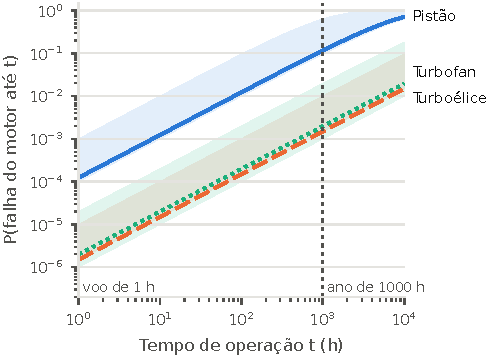
\includegraphics[width=\columnwidth]{figures/fig_prob_falha_tempo}
  \caption{Probabilidade de falha do motor até $t$. Linha: taxa nominal; faixa: da taxa mínima à máxima da Tabela~\ref{tab:taxas}.}
  \label{fig:tempo}
\end{figure}

Com as taxas nominais, o motor a pistão tem 83 vezes a probabilidade de falha do turboélice em um voo de 1~h e 62 vezes a do turbofan (Tabela~\ref{tab:metricas}).
Em um ano de 1000~h, a chance de ao menos uma falha é de 12\% no pistão e de 0,15\% a 0,20\% nos motores a turbina.
Mesmo no mínimo de sua faixa (10 \pcmh), o pistão falha 5 vezes mais que o turbofan e 10 vezes mais que o turboélice tomados no máximo das faixas deles (Fig.~\ref{fig:tempo}).
Entre os dois motores a turbina, o modelo não estabelece uma ordem: o turbofan tem taxa nominal um pouco maior, mas as faixas, de 0,15 a 1 e de 0,10 a 2 \pcmh, se sobrepõem quase por inteiro.

A redundância interna pouco altera o comportamento no tempo.
No pistão, a taxa equivalente fica em 12,40 \pcmh{} tanto em 1~h quanto em 1000~h, e o MTBF sem reparo (8026~h) fica perto do MTBF com o par restaurado a cada voo (8065~h).
Na análise de sensibilidade, a taxa total domina: quando $\lambda$ percorre a faixa, $F(1\,\mathrm{h})$ varia 10 vezes no pistão, 6,7 vezes no turboélice e 20 vezes no turbofan.
Já $\beta$ e $\lambda_u$ não mudam $F(1\,\mathrm{h})$, efeito da preservação da taxa publicada, e só alteram o Pareto.

\subsection{Subsistemas críticos}\label{sec:pareto}

\begin{figure*}[t]
  \centering
  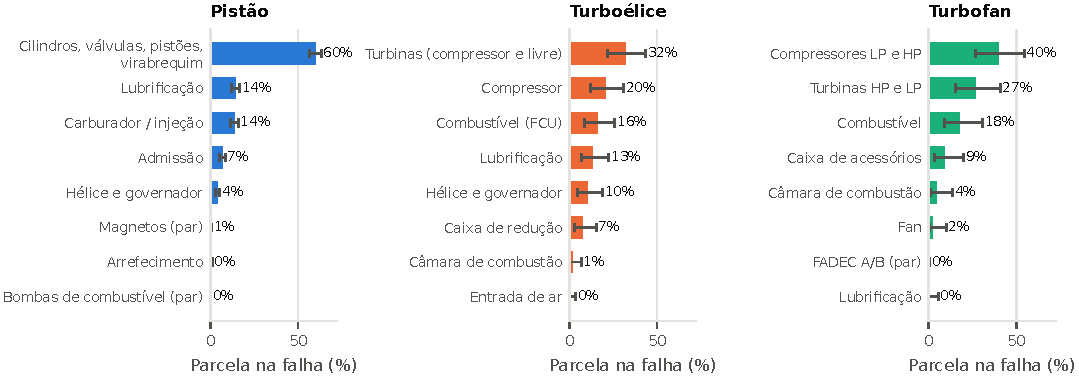
\includegraphics[width=\textwidth]{figures/fig_pareto_blocos}
  \caption{Parcela de cada subsistema na falha do motor em um voo de 1~h, com o intervalo de Jeffreys de 95\%.}
  \label{fig:pareto}
\end{figure*}

No pistão, o núcleo mecânico (cilindros, válvulas, pistões e virabrequim) responde por 60\% das falhas (IC 95\% de 57\% a 63\%), seguido de lubrificação e carburador/injeção, com 14\% cada (Fig.~\ref{fig:pareto}).
Com admissão e hélice, os cinco blocos em série sem redundância chegam a 99\%, como a proposta esperava.
Os pares redundantes ficam no fim do Pareto, com 0,6\% para os magnetos e 0,07\% para as bombas.
Nas turbinas, com 69 e 45 registros, os intervalos são largos. No turboélice, as turbinas lideram com 32\% (22\% a 43\%), seguidas do compressor, com 20\%, e do combustível (FCU), com 16\%.
No turbofan, lideram os compressores, com 40\% (27\% a 55\%), as turbinas, com 27\%, e o combustível, com 18\%; o fan, com um único registro, fica com 2\%.
Nos dois motores a turbina, as partes rotativas do gerador de gás concentram mais da metade das falhas.


\subsection{Redundância}\label{sec:redundancia}

\begin{table}[t]
  \caption{Efeito dos pares redundantes ($\beta=0{,}1$)}
  \label{tab:redundancia}
  \centering
  \setlength{\tabcolsep}{2.5pt}
  \begin{tabular}{@{}lrrcr@{}}
    \toprule
    Par & $n_p$ & $\lambda_u$ (\pcmh) & Ganho & Sem o par \\
    \midrule
    Magnetos (pistão) & 102 & 0,72 & 10$\times$ & +5,2\% \\
    Bombas (pistão) & 12 & 0,085 & 10$\times$ & +0,6\% \\
    FADEC A/B (turbofan) & 1 & 0,0022 & 10$\times$ & +1,0\% \\
    \bottomrule
    \multicolumn{5}{@{}l}{\footnotesize Ganho: $F$ de uma unidade sobre $F$ do par.} \\
    \multicolumn{5}{@{}l}{\footnotesize Sem o par: aumento em $F(1\,\mathrm{h})$ do motor.}
  \end{tabular}
\end{table}

Os pares reduzem em cerca de 10 vezes a probabilidade de perder a função (Tabela~\ref{tab:redundancia}).
O ganho é limitado por $\beta$: com $\beta=0{,}1$, quase toda a probabilidade de falha do par vem da causa comum, e o ganho fica perto de $1/\beta$.
Sem os dois pares, o motor a pistão teria uma probabilidade de falha em 1~h 5,8\% maior, $\num{1.31e-4}$ contra $\num{1.24e-4}$.
A coluna ``sem o par'' é também o risco de voar com uma unidade já inoperante: decolar com um magneto em pane eleva $F(1\,\mathrm{h})$ em 5,2\%, e com uma bomba em pane, em 0,6\%.
No turbofan, o FADEC tem um único registro, e a taxa da unidade vai de 0,0002 a 0,011 \pcmh{} no intervalo de Jeffreys; mesmo no máximo, a duplicação quase não altera o resultado.
Como falhas que o próprio par tolera raramente terminam em acidente, as taxas dos pares tendem a estar subestimadas.

\begin{figure}[t]
  \centering
  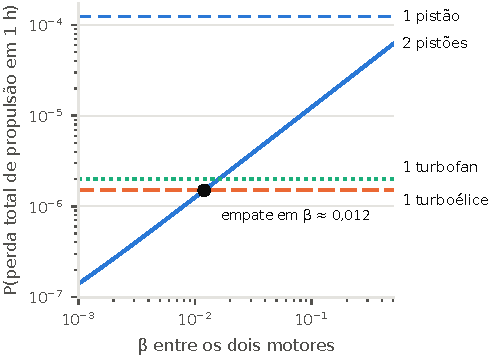
\includegraphics[width=\columnwidth]{figures/fig_bimotor}
  \caption{Probabilidade de perda total de propulsão em 1~h em função de $\beta$ entre os dois motores, com taxas nominais.}
  \label{fig:bimotor}
\end{figure}

Com dois motores, a perda total de propulsão exige que os dois falhem no mesmo voo.
Se as falhas fossem independentes, dois pistões perderiam toda a propulsão com probabilidade de $\num{1.5e-8}$ por hora, muito abaixo de um motor a turbina.
A causa comum entre os motores muda esse quadro (Fig.~\ref{fig:bimotor}).
Com as taxas nominais, o bimotor a pistão só é mais seguro que um turboélice se $\beta<0{,}012$, e mais seguro que um turbofan se $\beta<0{,}016$.
Com a taxa da turbina nos extremos da faixa, o limite vai de 0,012 a 0,081 contra o turboélice e de 0,008 a 0,161 contra o turbofan, na parte de baixo da faixa usual de $\beta$, de 0,01 a 0,3.
O bimotor também dobra a chance de ter alguma falha de motor no voo ($\num{2.5e-4}$ por hora), e o modelo conta só a perda total de propulsão, não a dificuldade de controlar o avião com um motor parado.

\subsection{Consequência da falha no NTSB}\label{sec:empirico}

\begin{figure}[t]
  \centering
  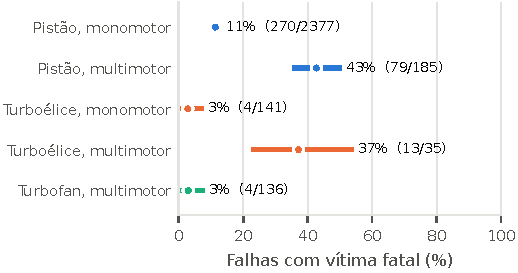
\includegraphics[width=\columnwidth]{figures/fig_ntsb_prob_fatal}
  \caption{Falhas de motor com vítima fatal no NTSB (2008--2026), por tecnologia e número de motores, com intervalo de Wilson de 95\%.}
  \label{fig:fatal}
\end{figure}

A Fig.~\ref{fig:fatal} dá uma medida empírica dessa dificuldade.
Nos multimotores a pistão, 43\% das falhas de motor registradas tiveram vítima fatal, contra 11\% nos monomotores; no turboélice, 37\% (13 de 35) contra 2,8\% (4 de 141).
A comparação é condicionada ao registro: no multimotor, a falha que termina em pouso normal raramente entra na base, enquanto no monomotor quase toda falha termina em pouso forçado.
Ainda assim, a falha de um motor de multimotor que chega ao NTSB é das mais graves, o que é coerente com a perda de controle por tração assimétrica, que o RBD não modela.
O monomotor turboélice tem a menor proporção (2,8\%), próxima à do turbofan (2,9\%).
Junto com o limite de $\beta$, isso indica que dois motores a pistão não equivalem, na prática, a um motor a turbina.
As falhas por combustível ficaram fora: são 1532 no pistão, 174 delas com vítima fatal.

\subsection{Taxa constante}\label{sec:weibull}

No pistão, com 903 casos e 4000 controles, a forma estimada pelo TSO é 0,99 (IC 95\% de 0,94 a 1,05; $p=0{,}79$ para $k=1$), compatível com a taxa constante do RBD entre revisões.
Pelo TSN, a forma é 1,08 (1,02 a 1,13), um desgaste leve ao longo da vida do motor: nos três quartis mais altos de TSN, a chance de falha é de 1,4 a 1,5 vez a do primeiro.
No turboélice, com 32 falhas com TSO, a forma é 1,28 (0,97 a 1,59), e no turbofan quase nenhum monomotor tem horas registradas.
O teste supõe que os controles tenham a idade de motor da frota.

\subsection{Limitações}\label{sec:limitacoes}

A estimativa por \eqref{eq:fracao} supõe que a chance de uma falha entrar no NTSB é a mesma para todos os blocos.
O NTSB registra sobretudo acidentes (no pistão, 2529 das 2562 falhas), e as frações descrevem as falhas que levaram a acidente ou incidente investigado, e não todas as falhas em voo.
Os 535 achados genéricos excluídos são supostos distribuídos entre os blocos na mesma proporção dos classificados.
Os motores entram por tipo, e não por modelo, e nas turbinas os blocos sem registro ficam com fração nula.
A taxa do turbofan vem do fabricante, e a do pistão mistura fabricantes e modelos da frota australiana, e não só o O-540.

\section{Conclusão}\label{sec:conclusao}

Decomposto em subsistemas, o modelo confirma a ordem de grandeza que a literatura atribui ao motor inteiro.
O pistão falha 62 a 83 vezes mais que os motores a turbina em um voo de 1~h, e a diferença resiste a toda a faixa de taxas publicadas.
Nele, 60\% das falhas estão no núcleo mecânico, que não tem redundância, e é ali que manutenção e projeto têm mais efeito; a ignição duplicada protege uma função que já respondia por pouco das falhas.
Nos motores a turbina, compressores e turbinas concentram as falhas, e o FADEC de dois canais quase não aparece nos registros.
A redundância não compensa a tecnologia: dois motores a pistão só superam uma turbina se a causa comum entre eles ficar abaixo de 1,2\% a 1,6\%, e, quando a falha de um motor de um multimotor a pistão chega ao NTSB, 43\% dos casos têm vítima fatal.
Entre turboélice e turbofan, as faixas da literatura não permitem estabelecer uma ordem.
O teste caso-controle com o tempo desde a revisão sustenta a taxa constante no pistão.

Três frentes ficam em aberto.
Obter horas voadas por frota permitiria a atualização Gama--Poisson das taxas absolutas, que a falta de exposição impediu.
Ampliar a base das turbinas, que têm 69 e 45 registros, estreitaria os intervalos do Pareto dessas tecnologias.
E taxas de remoção em campo das unidades redundantes, como magnetos e canais do FADEC, dariam um limite superior para $\lambda_u$, já que o NTSB só vê as falhas que terminam em acidente.


\bibliographystyle{IEEEtran-pt}
\bibliography{IEEEabrv,refs}

\end{document}
